\section{Gateway: Design \& Implementation}

\label{sec:gateway}
Having described our cryptographic building blocks, we can now discuss how they are used for encryption at the gateway.

\begin{figure}[t]
  \centering
  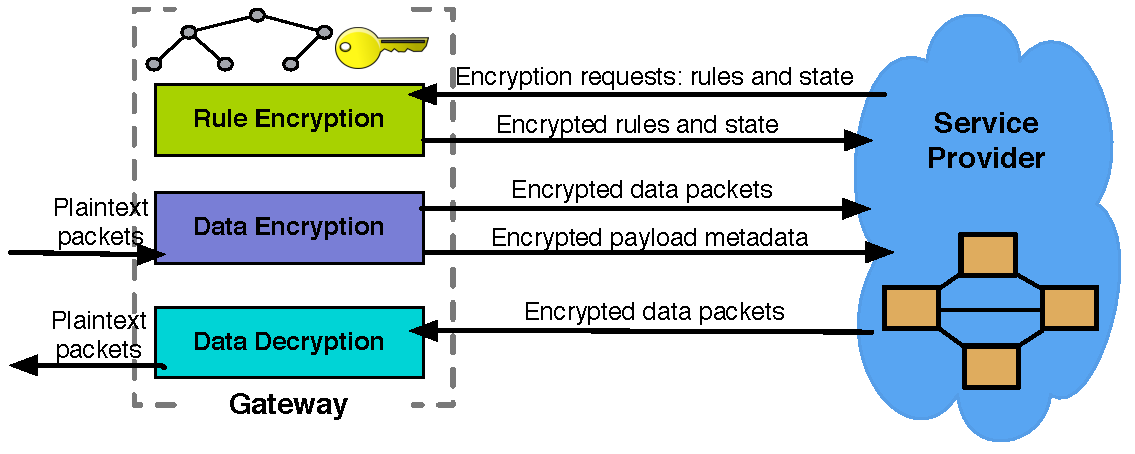
\includegraphics[width=3.25in]{fig/gateway2cloud}
  \caption[]{\label{fig:gatewaymeta} Communication between the cloud and gateway services: rule encryption, data encryption, and data decryption. \justine{Need to be consistent: is this a metadata channel or an extension channel}}
\end{figure}


\eat{
\begin{figure}[t]
  \centering
  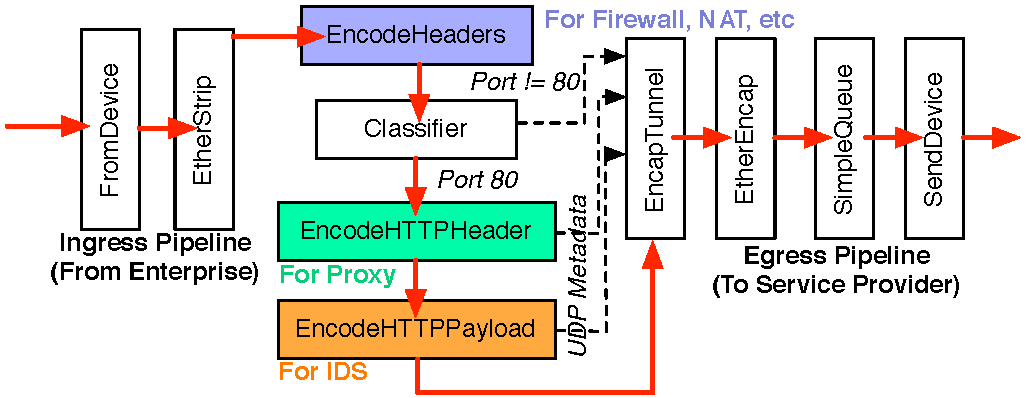
\includegraphics[width=3.25in]{fig/gatewaydiag}
  \caption[]{\label{fig:gateway} Data encryption (enterprise to cloud) click module.}
\end{figure}
}

The gateway serves two purposes. First, it redirects traffic to/from the cloud for middlebox processing. Second, it provides the cloud with encryptions of IDS/FW rulesets and updates to the RangeMatch tree.
Every gateway is configured statically to tunnel traffic to a fixed IP address at a single service provider point of presence.
A gateway can be logically thought of as three services: the rule encryption service, the pipeline from the enterprise to the cloud (Data encryption), and the pipeline from the cloud to the enterprise (Data decryption). 
All three services share access to the RangeMatch tree and the private key $k$.
Figure~\ref{fig:gatewaymeta} illustrates  these three services and the data they send to and from the cloud provider.

We design the gateway with two design principles in mind: 

\noindent{\bf Format-compatibility}: in converting plaintext traffic to encrypted traffic, the encrypted data should be structured in such a way that the traffic {\it appears as normal IPv6 traffic} to middleboxes performing the processing. This allows us to leave many middleboxes completely unmodified in how they perform per-packet operations, ensuring compatibility with optimizations including those in hardware (and hence good performance at the cloud). 

\noindent{\bf Low Complexity and Scalabibility}: the gateway should perform only inexpensive per-packet operations and should be parallelizable. The gateway should not require configuration other than to generate a key and establish a session with the cloud provider. If the gateway were as expensive and complex as the middleboxes themselves, the client would have no cost or management benefits from outsourcing. 

We now discuss how the gateway performs encryption and decryption (\S\ref{sec:dataenc}) and how rules are encyrpted (\S\ref{sec:rulenc}) with these design goals in mind.

\subsection{Data Encryption and Decryption}
\label{sec:dataenc}
\justine{Reiterate schemes.}
Data dedup.

\noindent{\bf IP and Transport Headers} are encrypted field by field (\eg{}, a source address in an input packet results in an encrypted source address field in the output packet) with RangeMatch.
We use RangeMatch for these fields because many middleboxes perform analysis over prefixes and ranges of values -- e.g., a firewall may block all connections from a restricted IP prefix.
RangeMatch also supports middleboxes like NATs and L4 Load Balancers, which rewrite a particular input value for an IP address or port to an output value for IP or port -- these `exact match' operations are a special case of RangeMatch, where the range being matched contains one value.
We store the AES encrypted values for the header fields in the options header; because RangeMatch is not reversible (it cannot be used to decrypt) we require these values to enable decryption when the packets leave the cloud and return to the gateway.

\noindent{\bf Payload Data} is encrypted with KeywordMatch using a searchable encryption approach (we discuss this in detail in \S\ref{sec:gateway}). This allows \sys to support DPI middleboxes, such as intrusion detection or exfiltration prevention.
These devices must detect whether or not there exists an exact match for an encrypted rule string {\it anywhere} in the connection bytestream.
The gateway transmits the encrypted bytestream over an `extension', secondary channel that only those middleboxes which perform DPI operations inspect. 
Other middleboxes ignore this extra data.
In addition, the payload is encrypted with AES and placed back into the packet payload -- like RangeMatch, KeywordMatch is not reversible and we require this data for decryption at the gateway.\justine{Do we? What if we just cached it at the gateway???}

\noindent{\bf HTTP Headers} are a special case of payload data.
Middleboxes such as proxies, L7 load balancers, and parental filters do not read arbitrary values from packet payloads: the only values they read are the HTTP headers.
We treat these values specially compared to other payload data; we encrypt the HTTP URI and METHOD and store them in IP options header of the packet containing the request.
As we will discuss in \S\ref{sec:gatewayarch}, supporting middleboxes which operate over payload data in general requires a stateful gateway; we can keep our gateway stateless for those middleboxes which {\it only} access HTTP headers in the payload by storing these values in the options header. 



\subsection{Rule Encryption}
\label{sec:rulenc}


The rule encryption component provides the cloud provider with encrypted rules/policies to use at the middlebox. 
There are two possible ways rules can be generated. First, an enterprise may choose to generate their own rules, in which case, they send encrypted versions of the rules directly to the cloud.
Alternately, the enterprise may opt in to a `default' set of rules from the cloud provider, in which case the cloud provider sends the rules to the gateway which encrypts them and sends them back.
Rules can contain IP and transport header values -- which must be encrypted with RangeMatch -- or HTTP header fields, or DPI signatures, which must be encrypted with KeywordMatch.

The rule encryption component also handles rule updates. 
Whenever an adjustment is made to the RangeMatch table, it sends an update to the cloud provider with the adjusted mappings/rules.
If the gateway ever changes its key, the encryption component must also signal to the cloud provider and re-encrypt all rules.


\subsection{Discussion}
\label{sec:gwdiscuss}
\textbf{Scalability}
\textbf{Complexity}
\textbf{Fault Tolerance}
